%----------------------------------------
\documentclass[aps, prl]{revtex4-2}  % for review and submission
%\usepackage{graphicx}  % needed for figures
%\usepackage{dcolumn}   % needed for some tables
%\usepackage{bm}        % for math
%\usepackage{amssymb}   % for math
%\usepackage[hidelinks]{hyperref}
%\usepackage{fancyhdr}
%\usepackage{xcolor}
%\usepackage{grffile}
%\usepackage[top=1in,left=0.8in, right=0.8in, bottom=0.8in]{geometry}
%\usepackage{float}
%\usepackage[compact]{titlesec}
%\titlespacing{\section}{0pt}{2ex}{2ex}

\usepackage{graphicx}  % needed for figures
\usepackage{ragged2e}
\usepackage{dcolumn}   % needed for some tables
\usepackage{bm}        % for math
\usepackage{amssymb}   % for math
\usepackage{amsmath}   % for math
\usepackage[top=0.85in,left=0.9in, right=0.9in, bottom=0.9in]{geometry}
\usepackage[hidelinks]{hyperref}
\usepackage{fancyhdr}
\usepackage{xcolor}
\usepackage{float}
\usepackage{lipsum}
\usepackage[compact]{titlesec}

\hypersetup{
    colorlinks,
    linkcolor={blue!80!black},
    citecolor={blue!80!black},
    urlcolor={blue!80!black}
}
% avoids incorrect hyphenation, added Nov/08 by SSR
\hyphenation{ALPGEN}
\hyphenation{EVTGEN}
\hyphenation{PYTHIA}
%

\begin{document}
\title{Supplementary Materials: Probing the Deuteron at Very Large Internal Momenta}
\maketitle
\section{\large Spectrometer Acceptance}
\noindent The $^{1}$H$(e,e'p)$ coincidence elastic reaction was used (at kinematics very similar to the deuteron 80 MeV/c setting) to check of the spectrometers'
acceptance model\cite{COSY} using the simulation program, SIMC. The proton form factor parametrization of Ref.\cite{PhysRevC.69.022201} were used. \\
\indent Figures \ref{fig:fig1} and \ref{fig:fig2} show the spectrometers' reconstructed quantities ($\delta$,  $Y_{\mathrm{tar}}$, $Y'_{\mathrm{tar}}$, $X'_{\mathrm{tar}}$)
where $\delta$ is the momentum fraction defined as $\delta = \frac{P-P_{0}}{P_{p}}$, where $P$ is the particle momentum and $P_{0}$ is the spectrometer central momentum.
The $Y_{\mathrm{tar}}$ is the reconstructed trajectory along the spectrometer $y-$coordinate, and ($Y'_{\mathrm{tar}}$, $X'_{\mathrm{tar}}$) are the reconstructed trajectories
tangent to the spectrometer central axis ($+z$) and are defined as $Y'_{\mathrm{tar}} = \frac{dY_{\mathrm{tar}}}{dz}$ and $X'_{\mathrm{tar}} = \frac{dX_{\mathrm{tar}}}{dz}$.
See Section 4.4 of Ref.\cite{cyero_phdthesis} for a more detailed description of these quantities.\\
\begin{figure}[h]
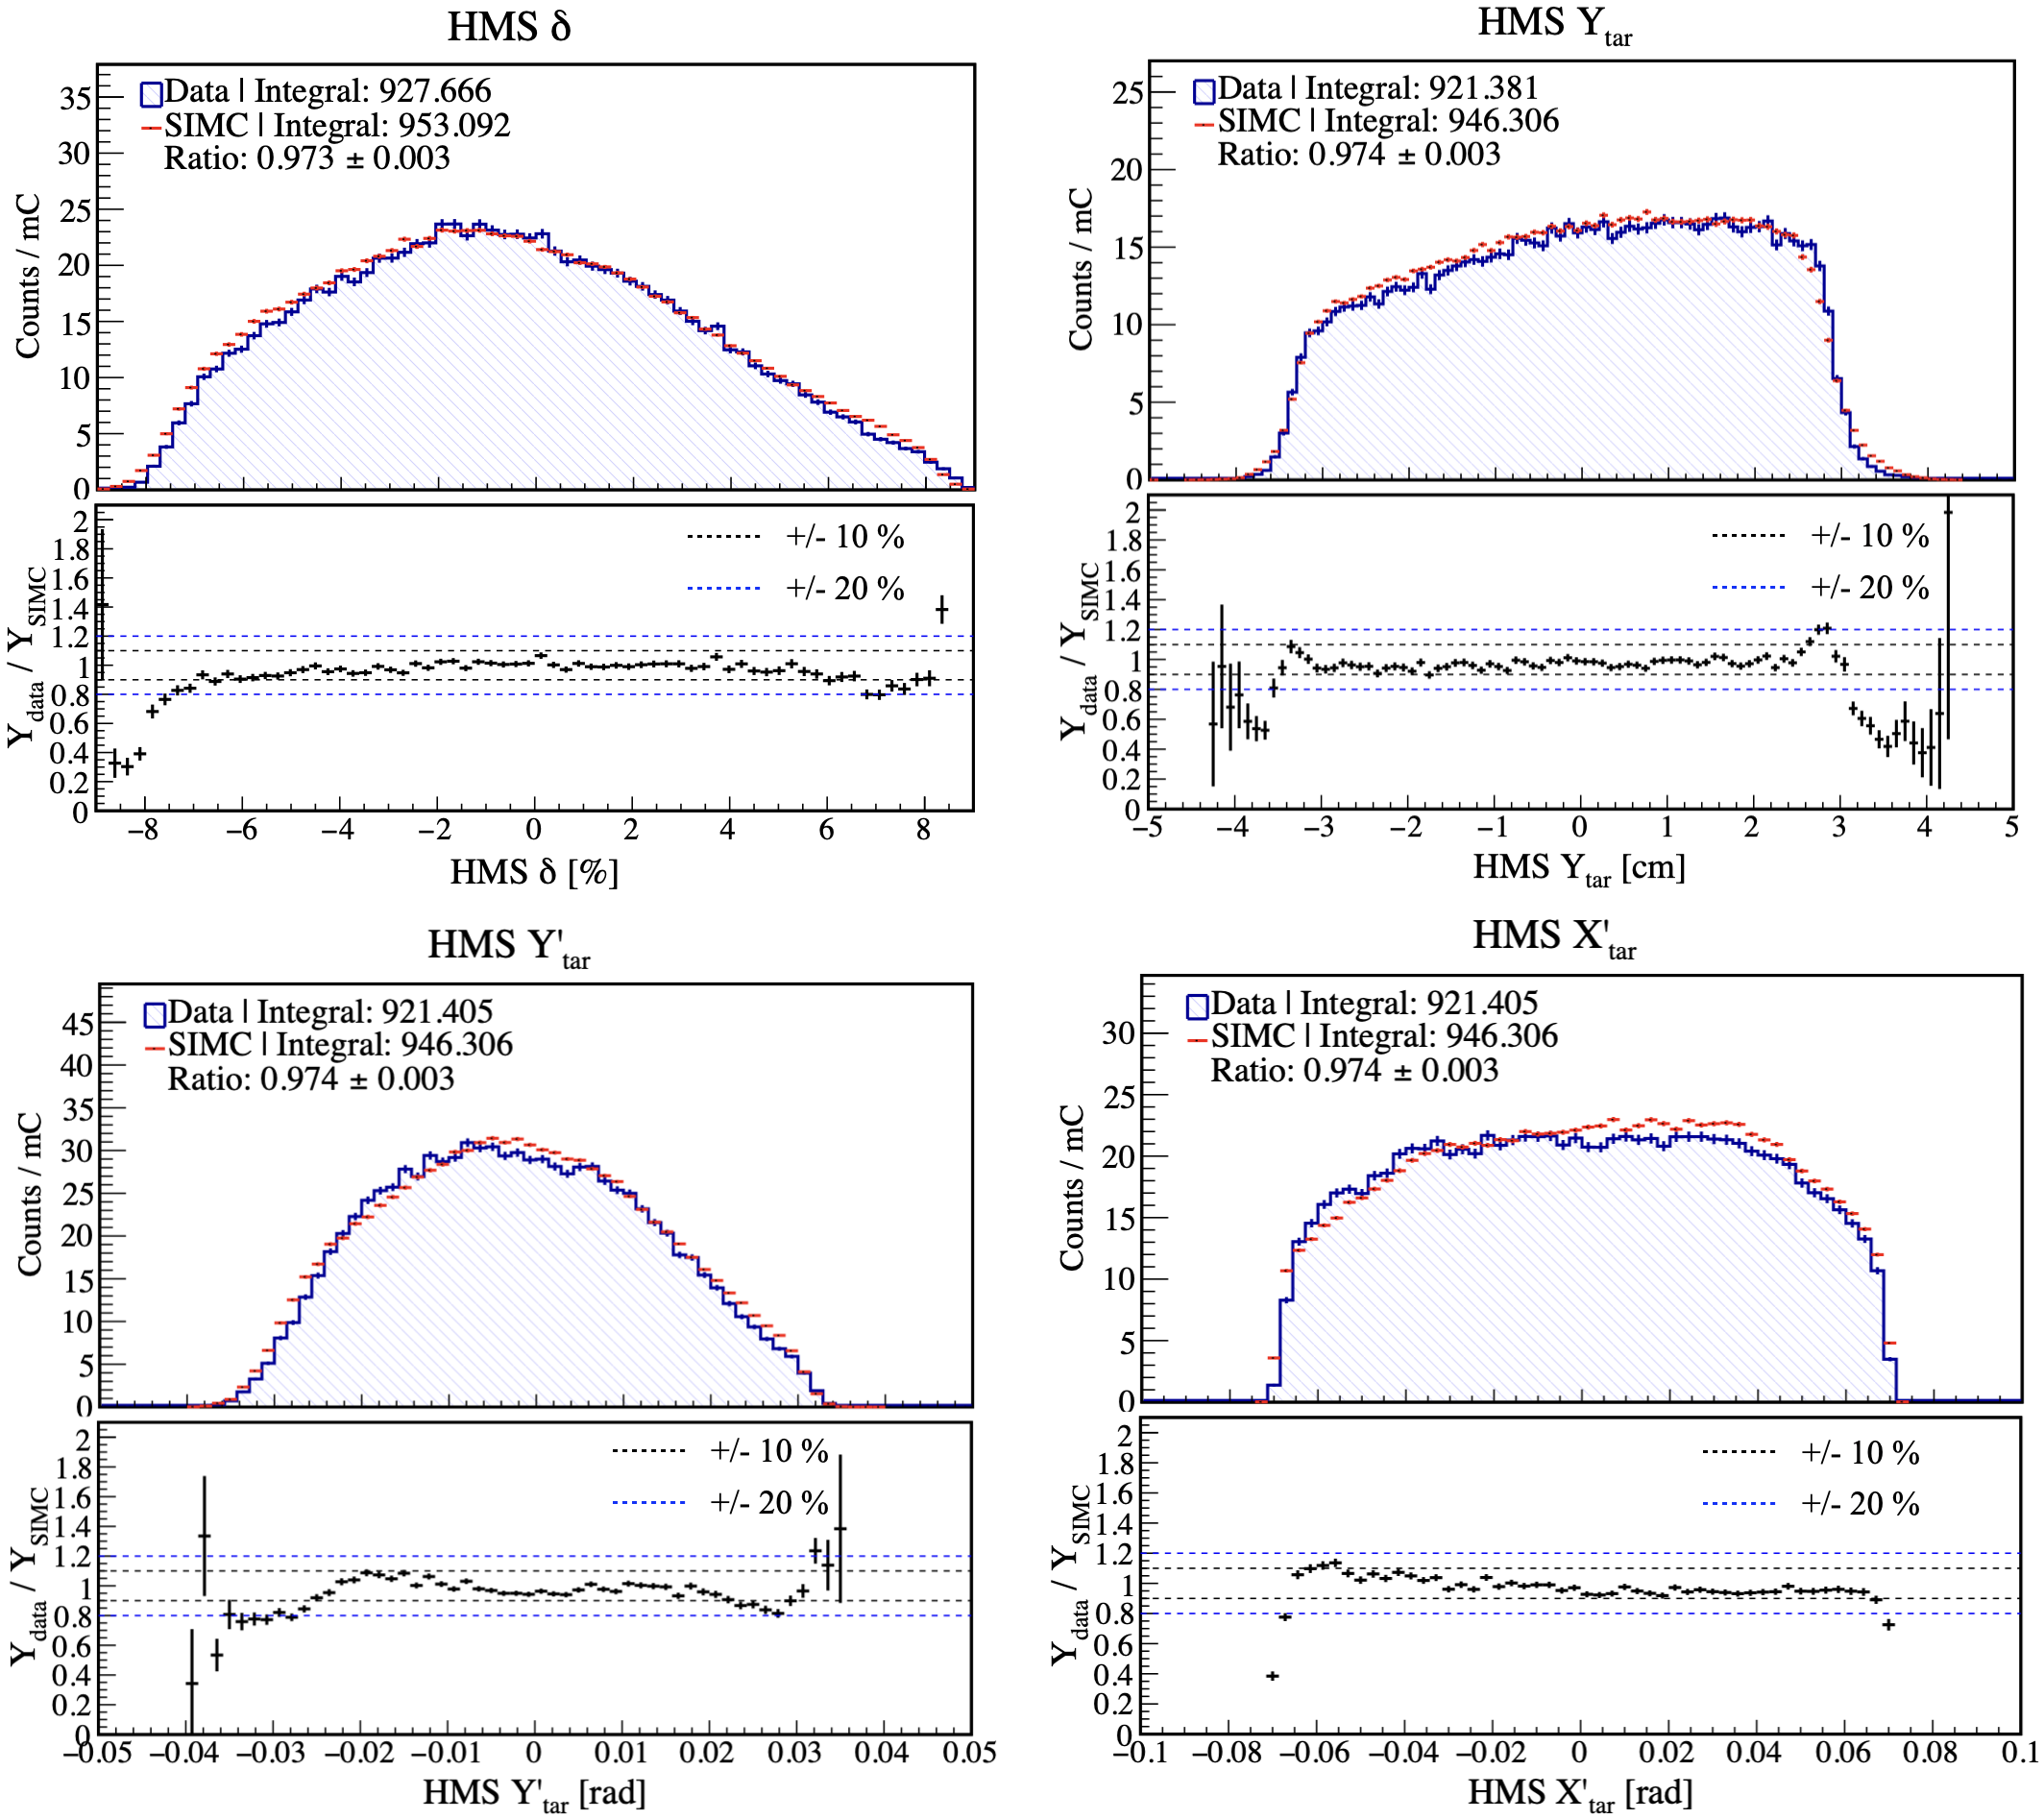
\includegraphics[scale=0.36]{plots/hms_acc_3288.png}
\caption{HMS reconstructed quantities ($\delta$,  $Y_{\mathrm{tar}}$, $Y'_{\mathrm{tar}}$, $X'_{\mathrm{tar}}$) at the target reaction vertex using $^{1}$H$(e,e'p)$.
  For each reconstructed quantity, the top panel shows a comparison between data (blue) and SIMC (red) with their respective integrated charge-normalized yields
  and the data-to-SIMC ratio numerical values (top-left). The bottom panel shows the ratio of the data (Y$_{\mathrm{data}}$) to SIMC (Y$_{\mathrm{SIMC}}$) on a bin-by-bin basis, where the inner (black)
and outer (blue) dashed lines represent a percent deviation from unity of $\pm10\%$ and $\pm20\%$, respectively.}
\label{fig:fig1}
\end{figure}
\clearpage
\begin{figure}[!ht]
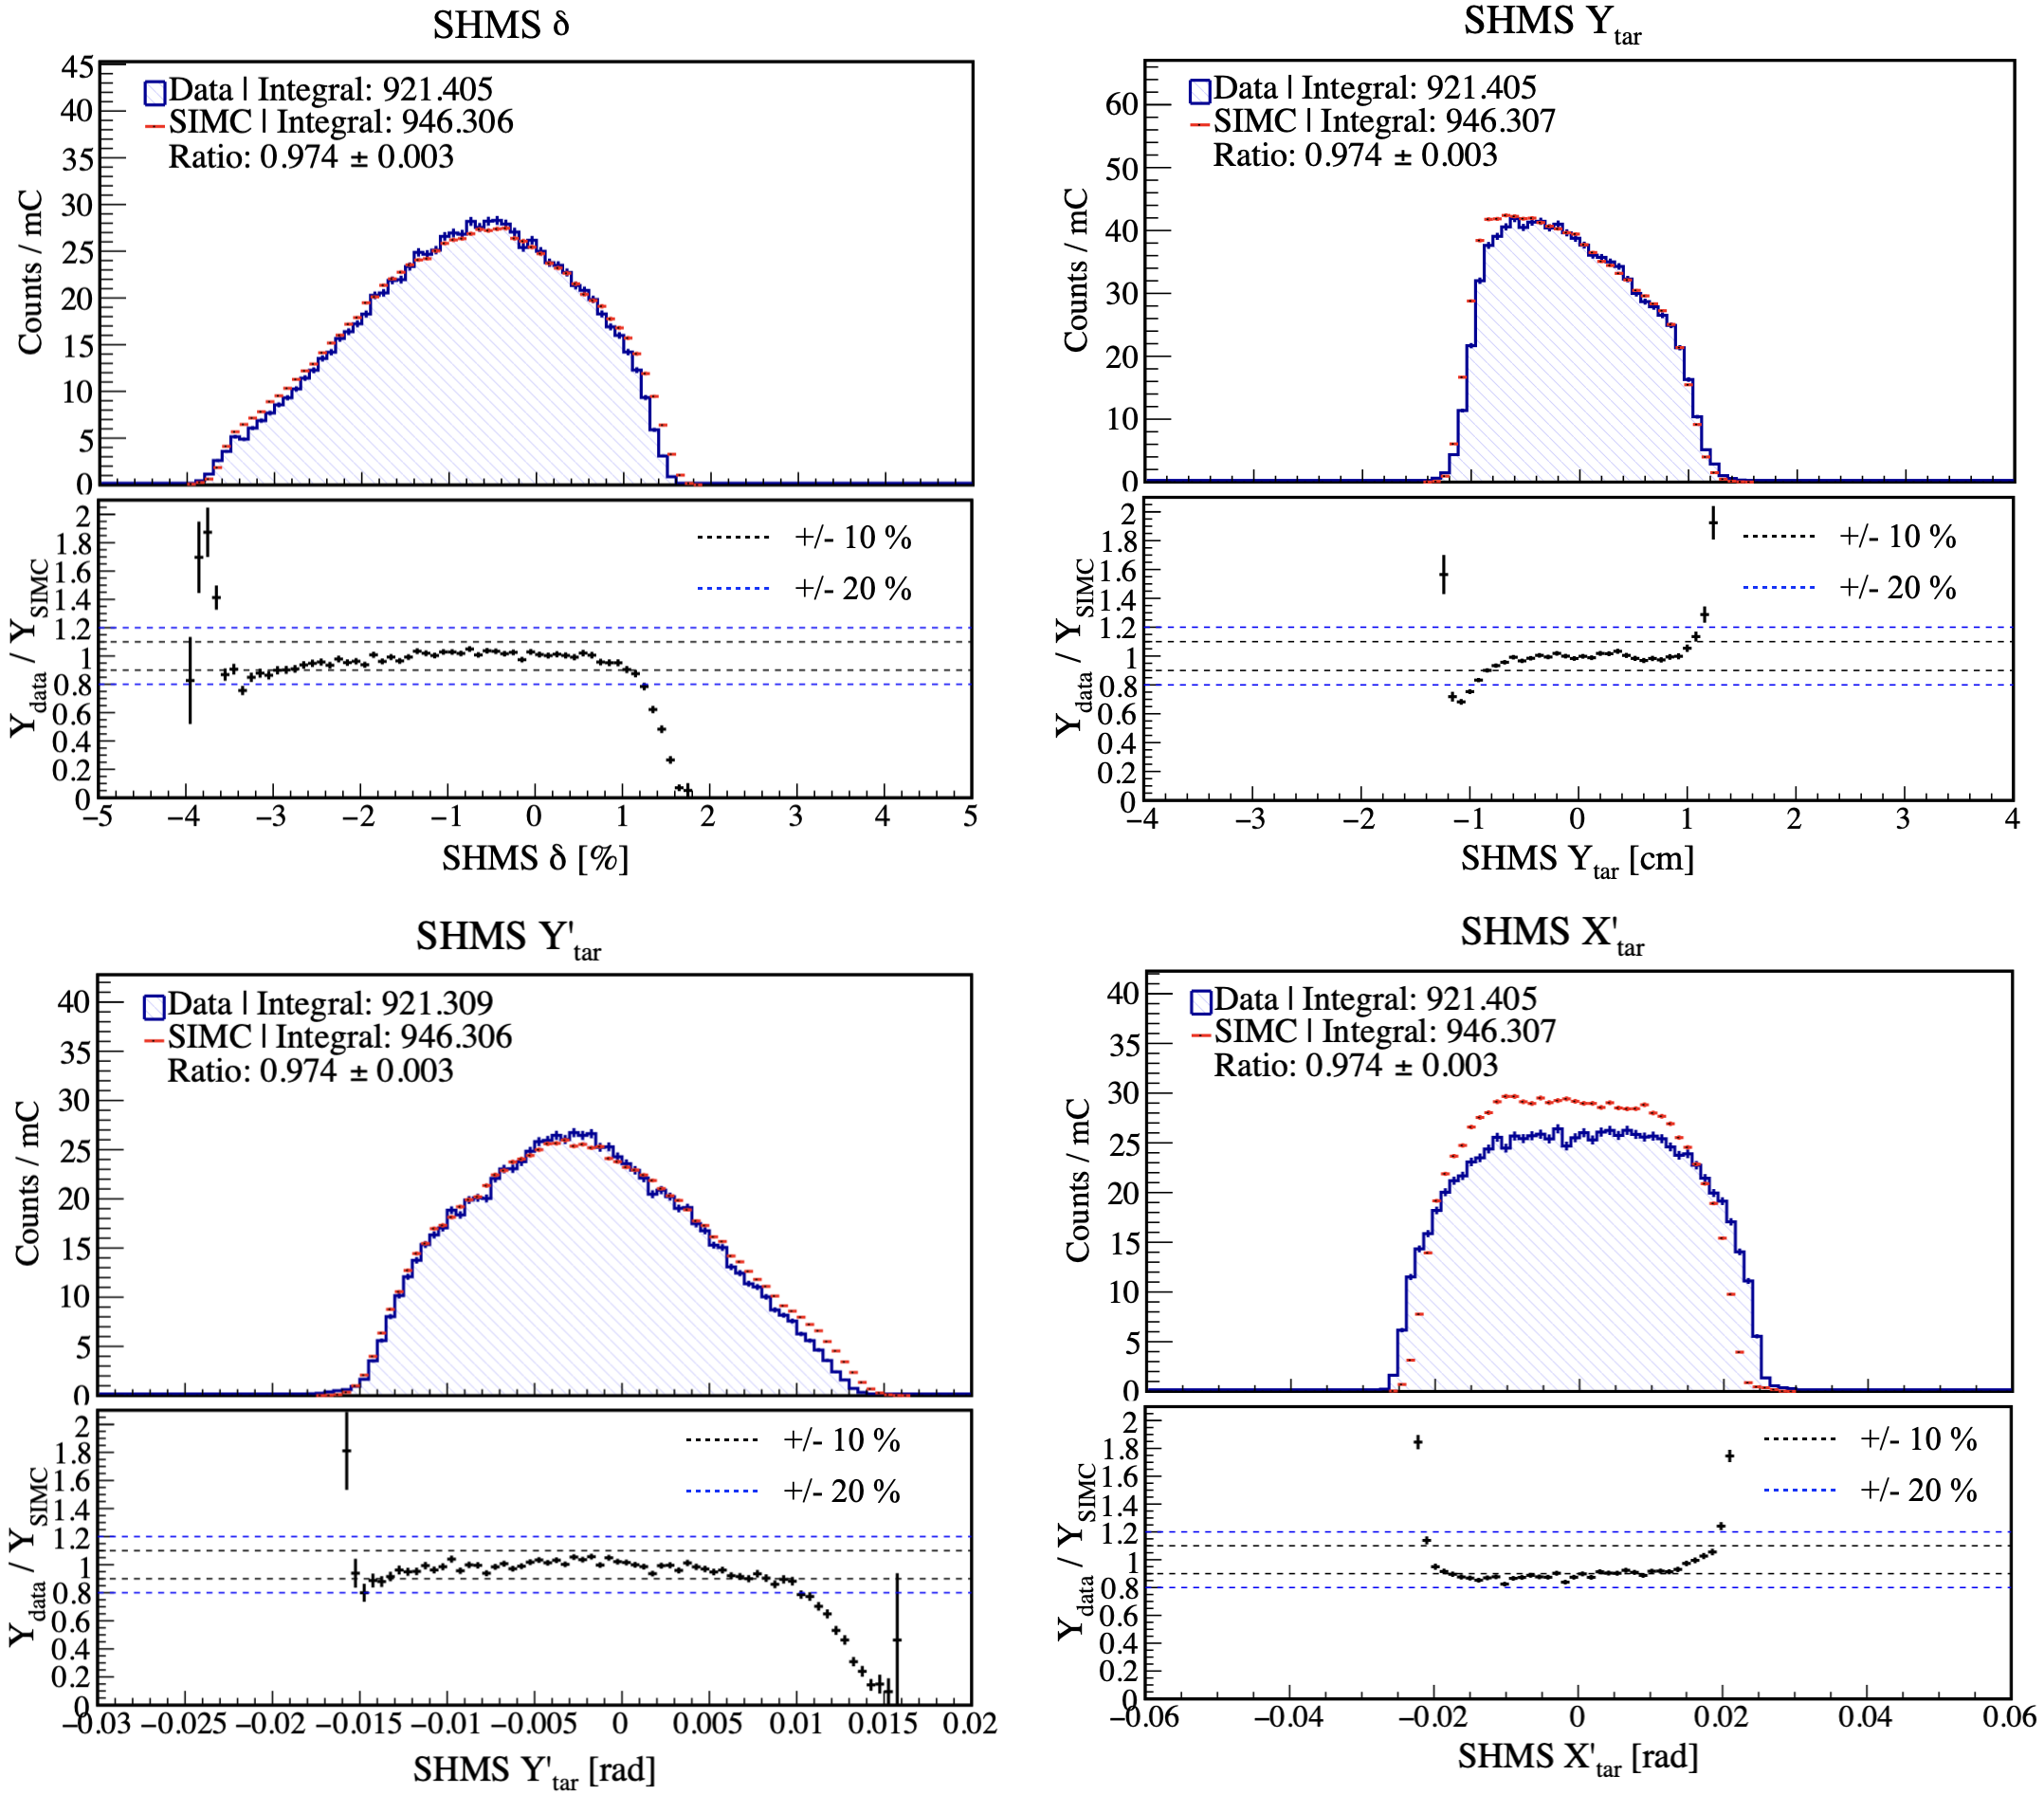
\includegraphics[scale=0.36]{plots/shms_acc_3288.png}
\caption{Same as Fig. \ref{fig:fig1}, but for SHMS. }
\label{fig:fig2}
\end{figure}
\section{\large Event Selection Cuts}
\noindent Figures \ref{fig:fig3}-\ref{fig:fig7} show the event selection cuts for data (blue hatched) and SIMC (red data points) for the deuteron 80 MeV/c kinematic setting at $\theta_{nq}=35\pm5^{\circ}$.
The black dashed or red solid lines (for collimators) represent the cuts or geometrical (collimators) boundaries used to select true $^{2}$H$(e,e'p)n$ coincidence events.
The exact same cuts were also applied to the 580 and 750 MeV/c settings. The data yield has been normalized by the total charge and corrected for the inefficiencies described in the Letter.
The FSI model from J.M. Laget was used in the simulation for the plots shown below.
\begin{figure}[!h]
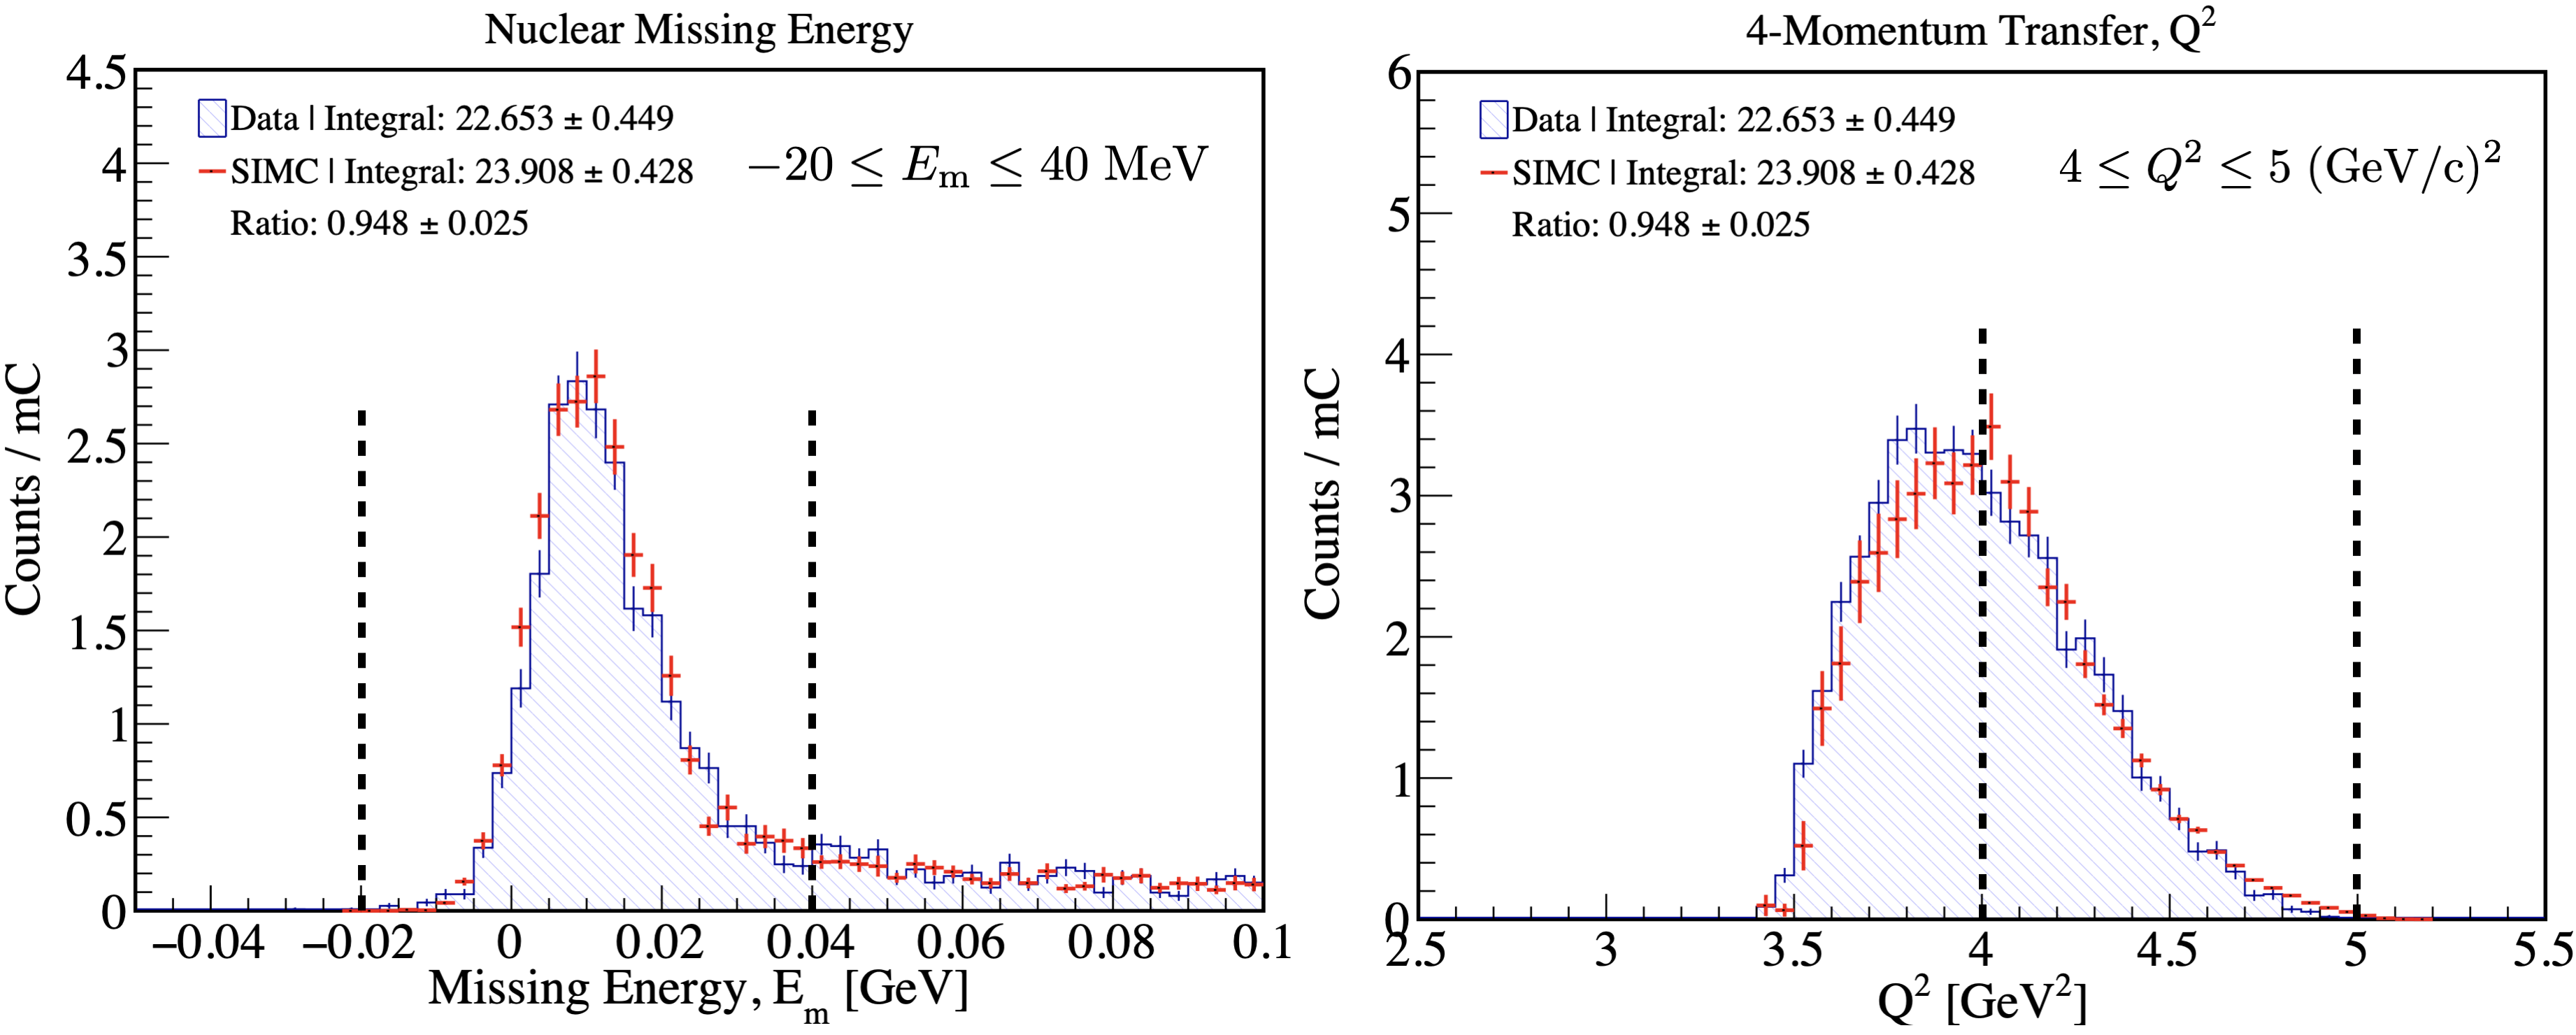
\includegraphics[scale=0.30]{plots/Em_and_Q2_CUT_80MeV_35deg.png}
\caption{Event selection cuts on missing energy (left) and 4-momentum transfer (right).}
\label{fig:fig3}
\end{figure}
\clearpage
\begin{figure}
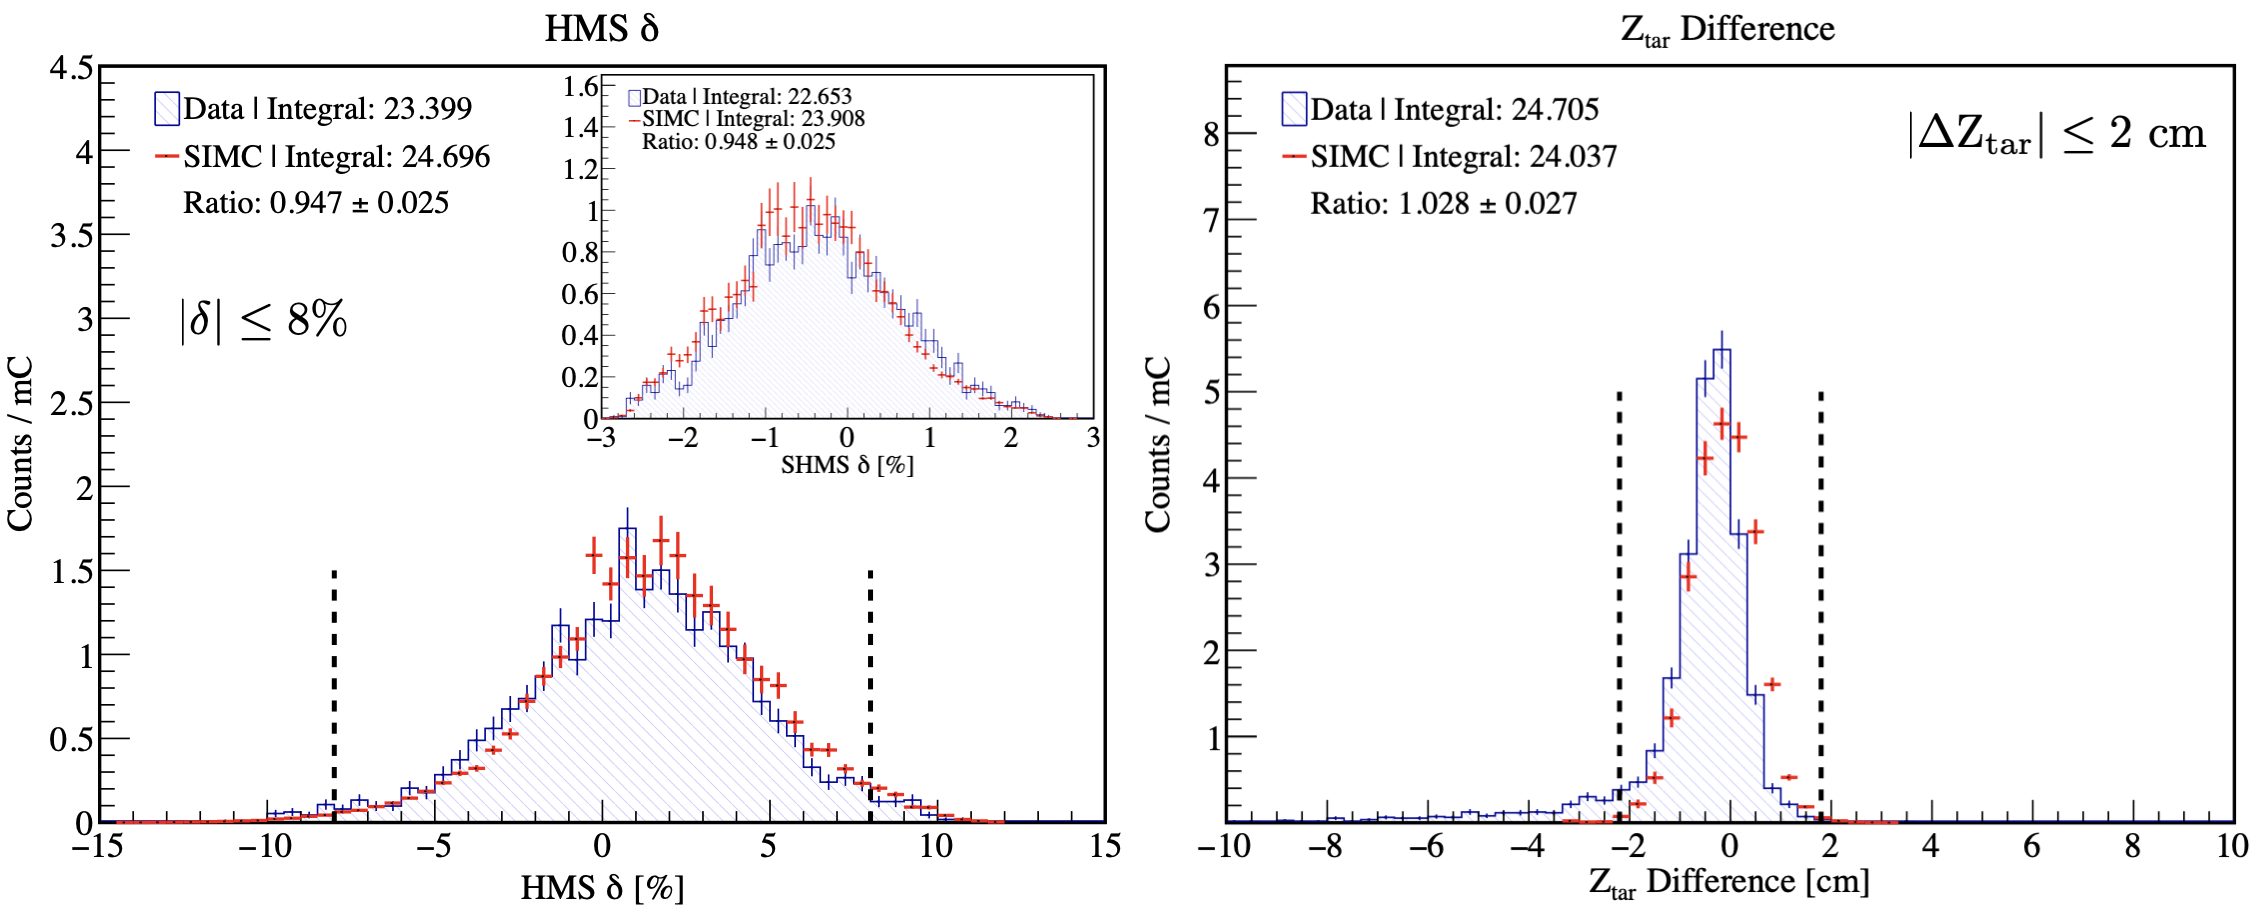
\includegraphics[scale=0.30]{plots/deltaAcc_and_ZtarCUT_80MeV_35deg.png}
\caption{Acceptance cut on HMS momentum fraction (left) and event selection cut on the difference between the $z$-reaction vertex on both spectrometers (right).
  Inset (left): The SHMS momentum fraction was set by the HMS $\delta$ cut to be $\lesssim$3$\%$ which is well within the SHMS specifications of  $-10 \leq \delta \leq22 \%$}
\label{fig:fig4}
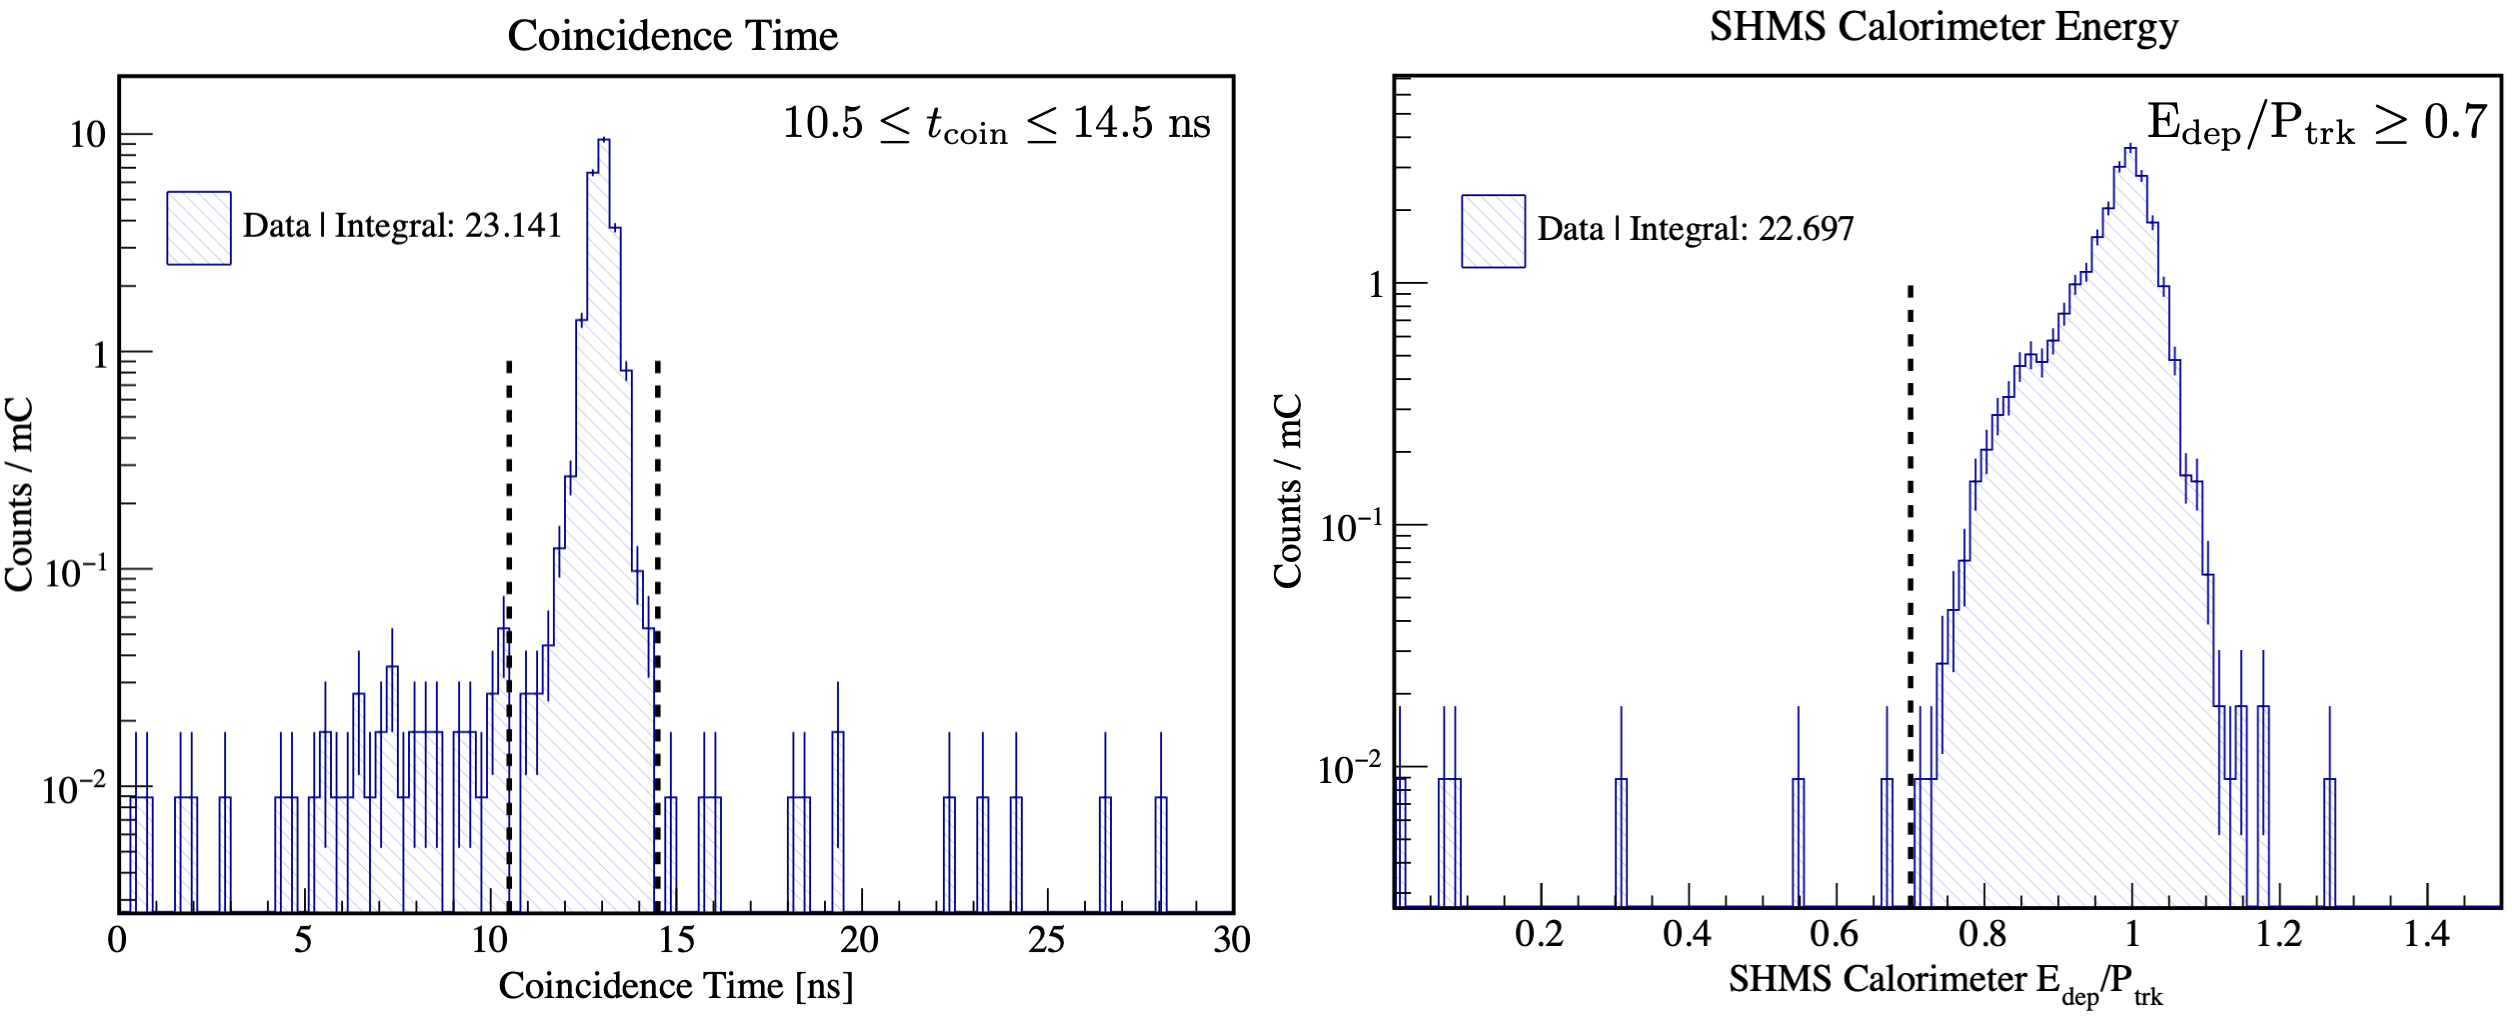
\includegraphics[scale=0.30]{plots/coin_and_eCal_CUT_80MeV_35deg.png}
\caption{Event selection cuts on the $ep$ coincidence time (left) and total deposited energy on calorimeted normalized by the track momentum (right).}
\label{fig:fig5}
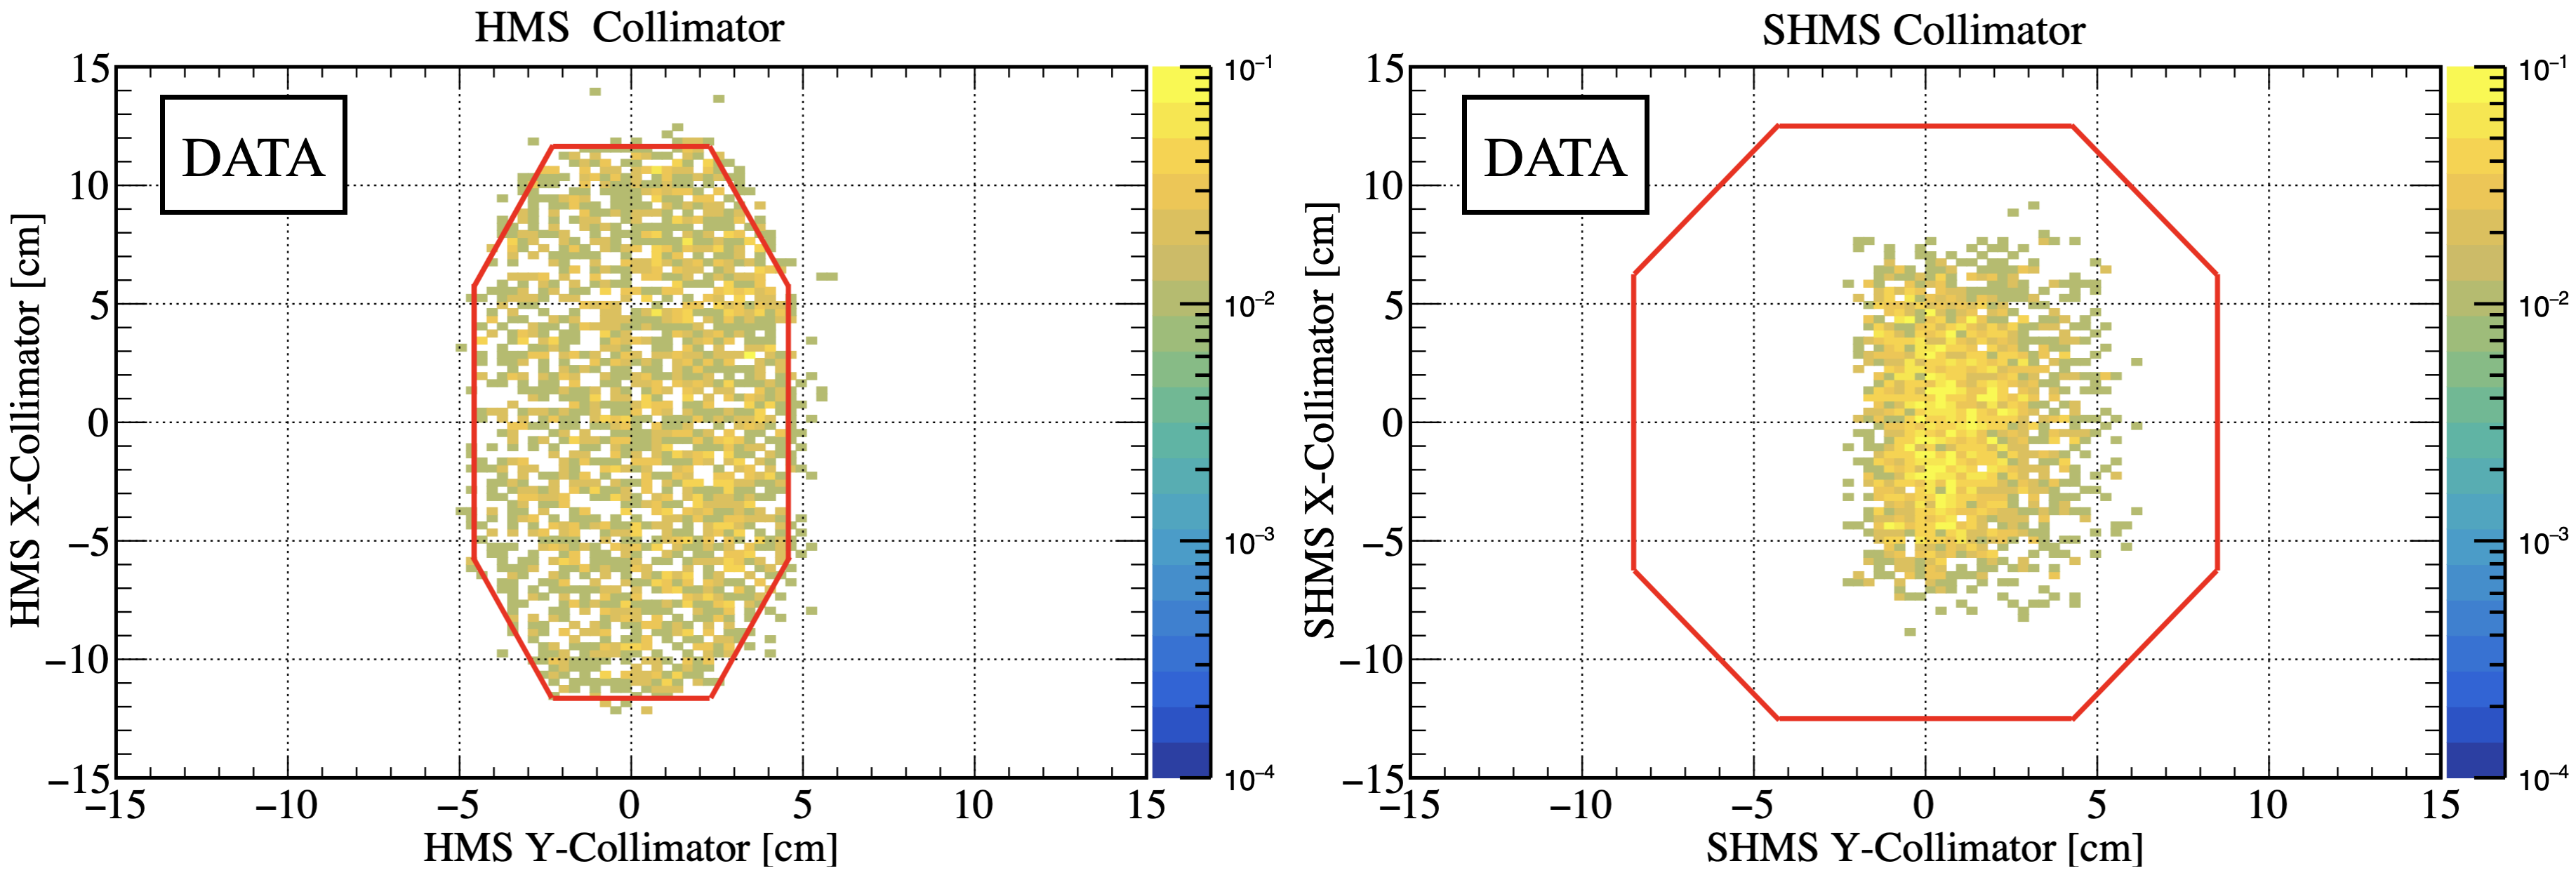
\includegraphics[scale=0.30]{plots/collimator_CUT_80MeV_35deg_data.png}
\caption{Geometrical acceptance cut on reconstructed events projected at the HMS collimator (left). The SHMS events (in coincidence with HMS events) were projected at the SHMS collimator (right)
  which clearly shows that the acceptance of the SHMS is driven by that of the HMS.}
\label{fig:fig6}
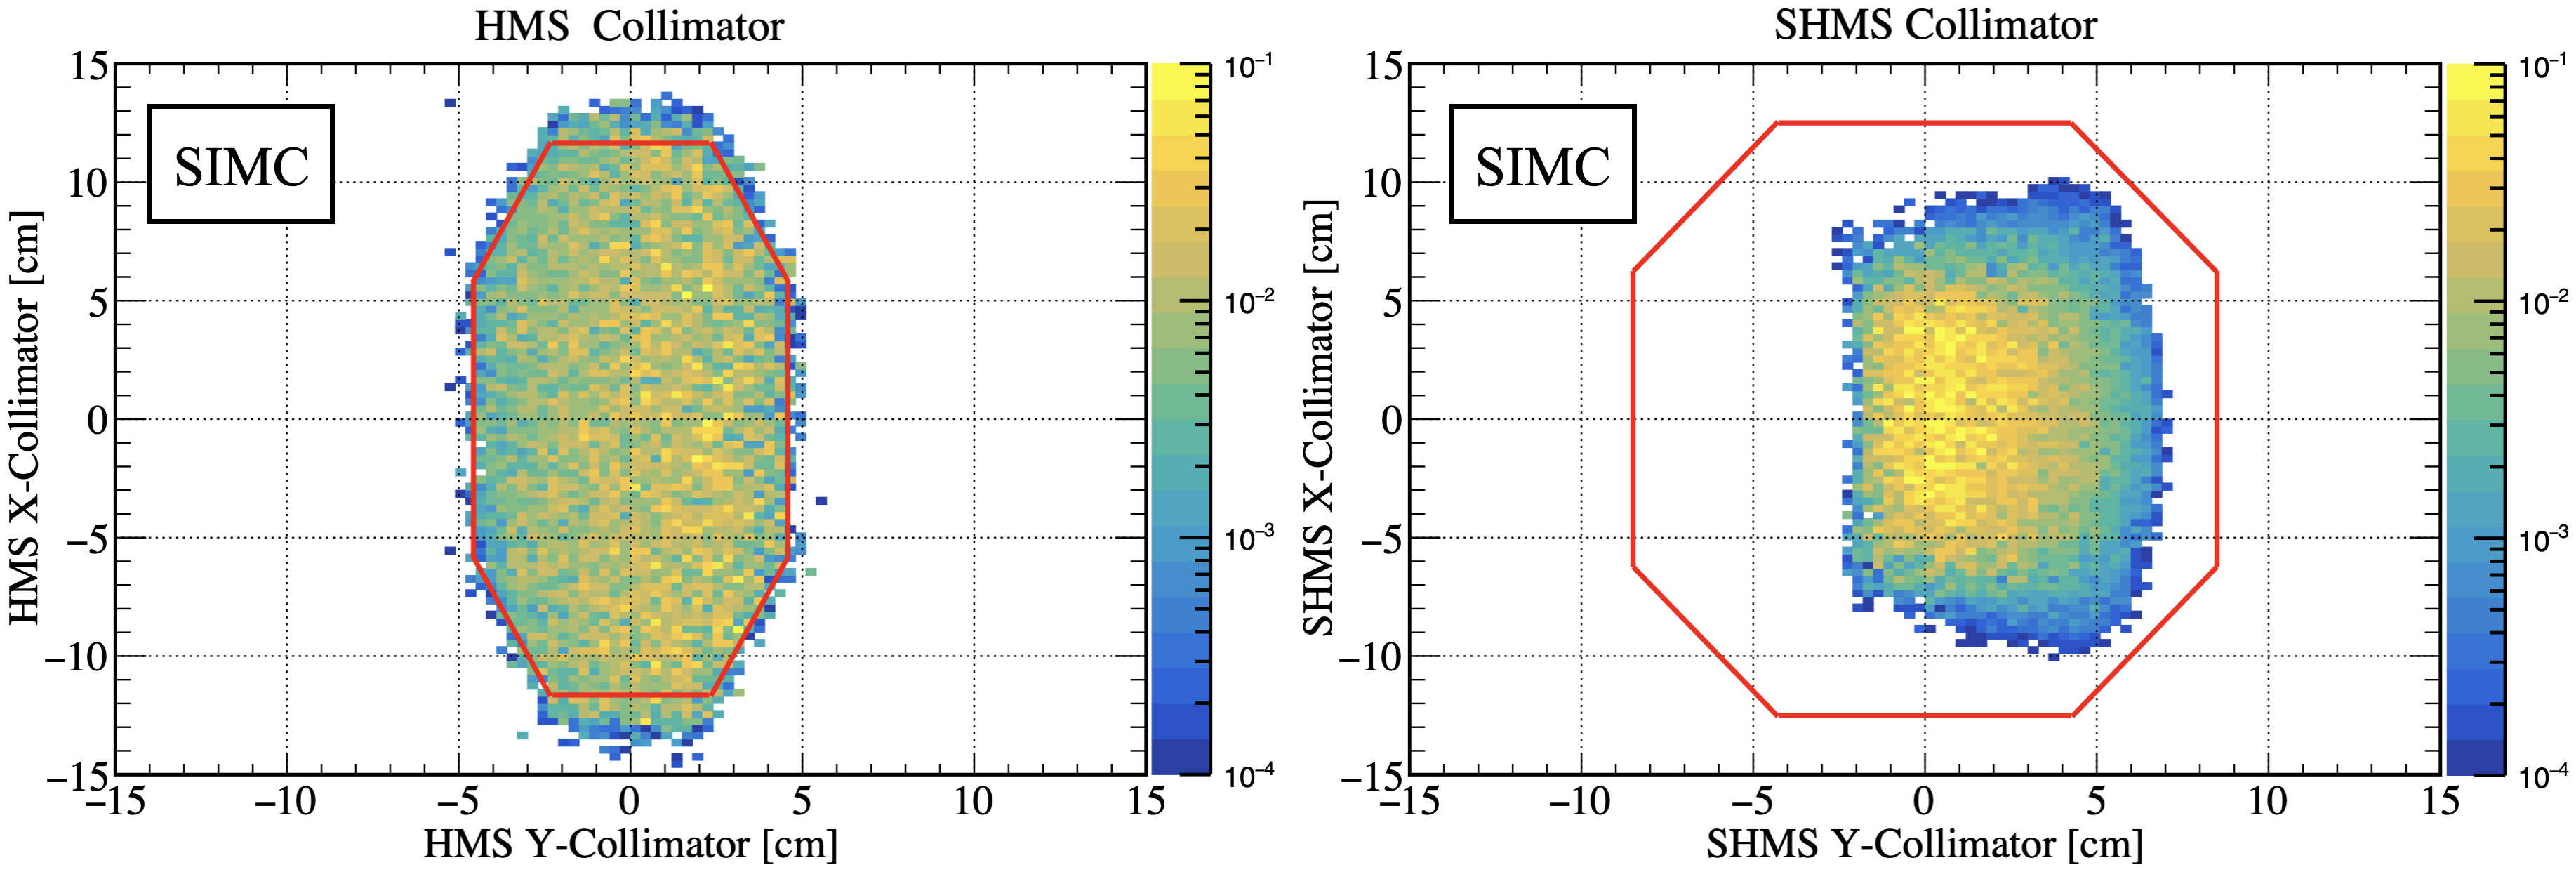
\includegraphics[scale=0.30]{plots/collimator_CUT_80MeV_35deg_SIMC.png}
\caption{Same as Fig. \ref{fig:fig6}, but for simulation.}
\label{fig:fig7}
\end{figure}
\clearpage
\section{\large Estimate of the Target Cell Endcaps Contribution to the Data Yield}
\noindent To estimate the contribution to the yield due to the electron interaction with the aluminum endcaps of the target cell,
a sample of events were selected in the negative part of the missing energy spectrum using the deuteron high missing momentum settings (580 and 750 MeV/c).
%This was only made possible due to the high recoil kinetic energies reconstructed at these kinematics. For electron interactions with the aluminum target endcaps,
%the reconstructed events extended to the negative part of the missing energy spectrum since we assume the mass of the deuteron in the missing energy definition.\\
We assume that the contribution due to the target endcaps is constant across the missing energy spectrum, therefore, by selecting a sample in the
negative part of the spectrum over a specific range, we can estimate the endcaps contribution beneath the deuteron missing energy peak over the same range.\\
\indent Figure \ref{fig:fig8} shows the missing energy spectrum for the 580 MeV/c setting (left) and the corresponding reconstructed SHMS $z$-vertex (right) for the specified
range. The integral over endcaps and $^{2}\mathrm{H}(e,e'p)n$ events show that the contribution from the cell walls is 0.00806/0.275 $\sim$ 0.0293 or approximately 2.9 $\%$
which is negligible.
\begin{figure}[!h]
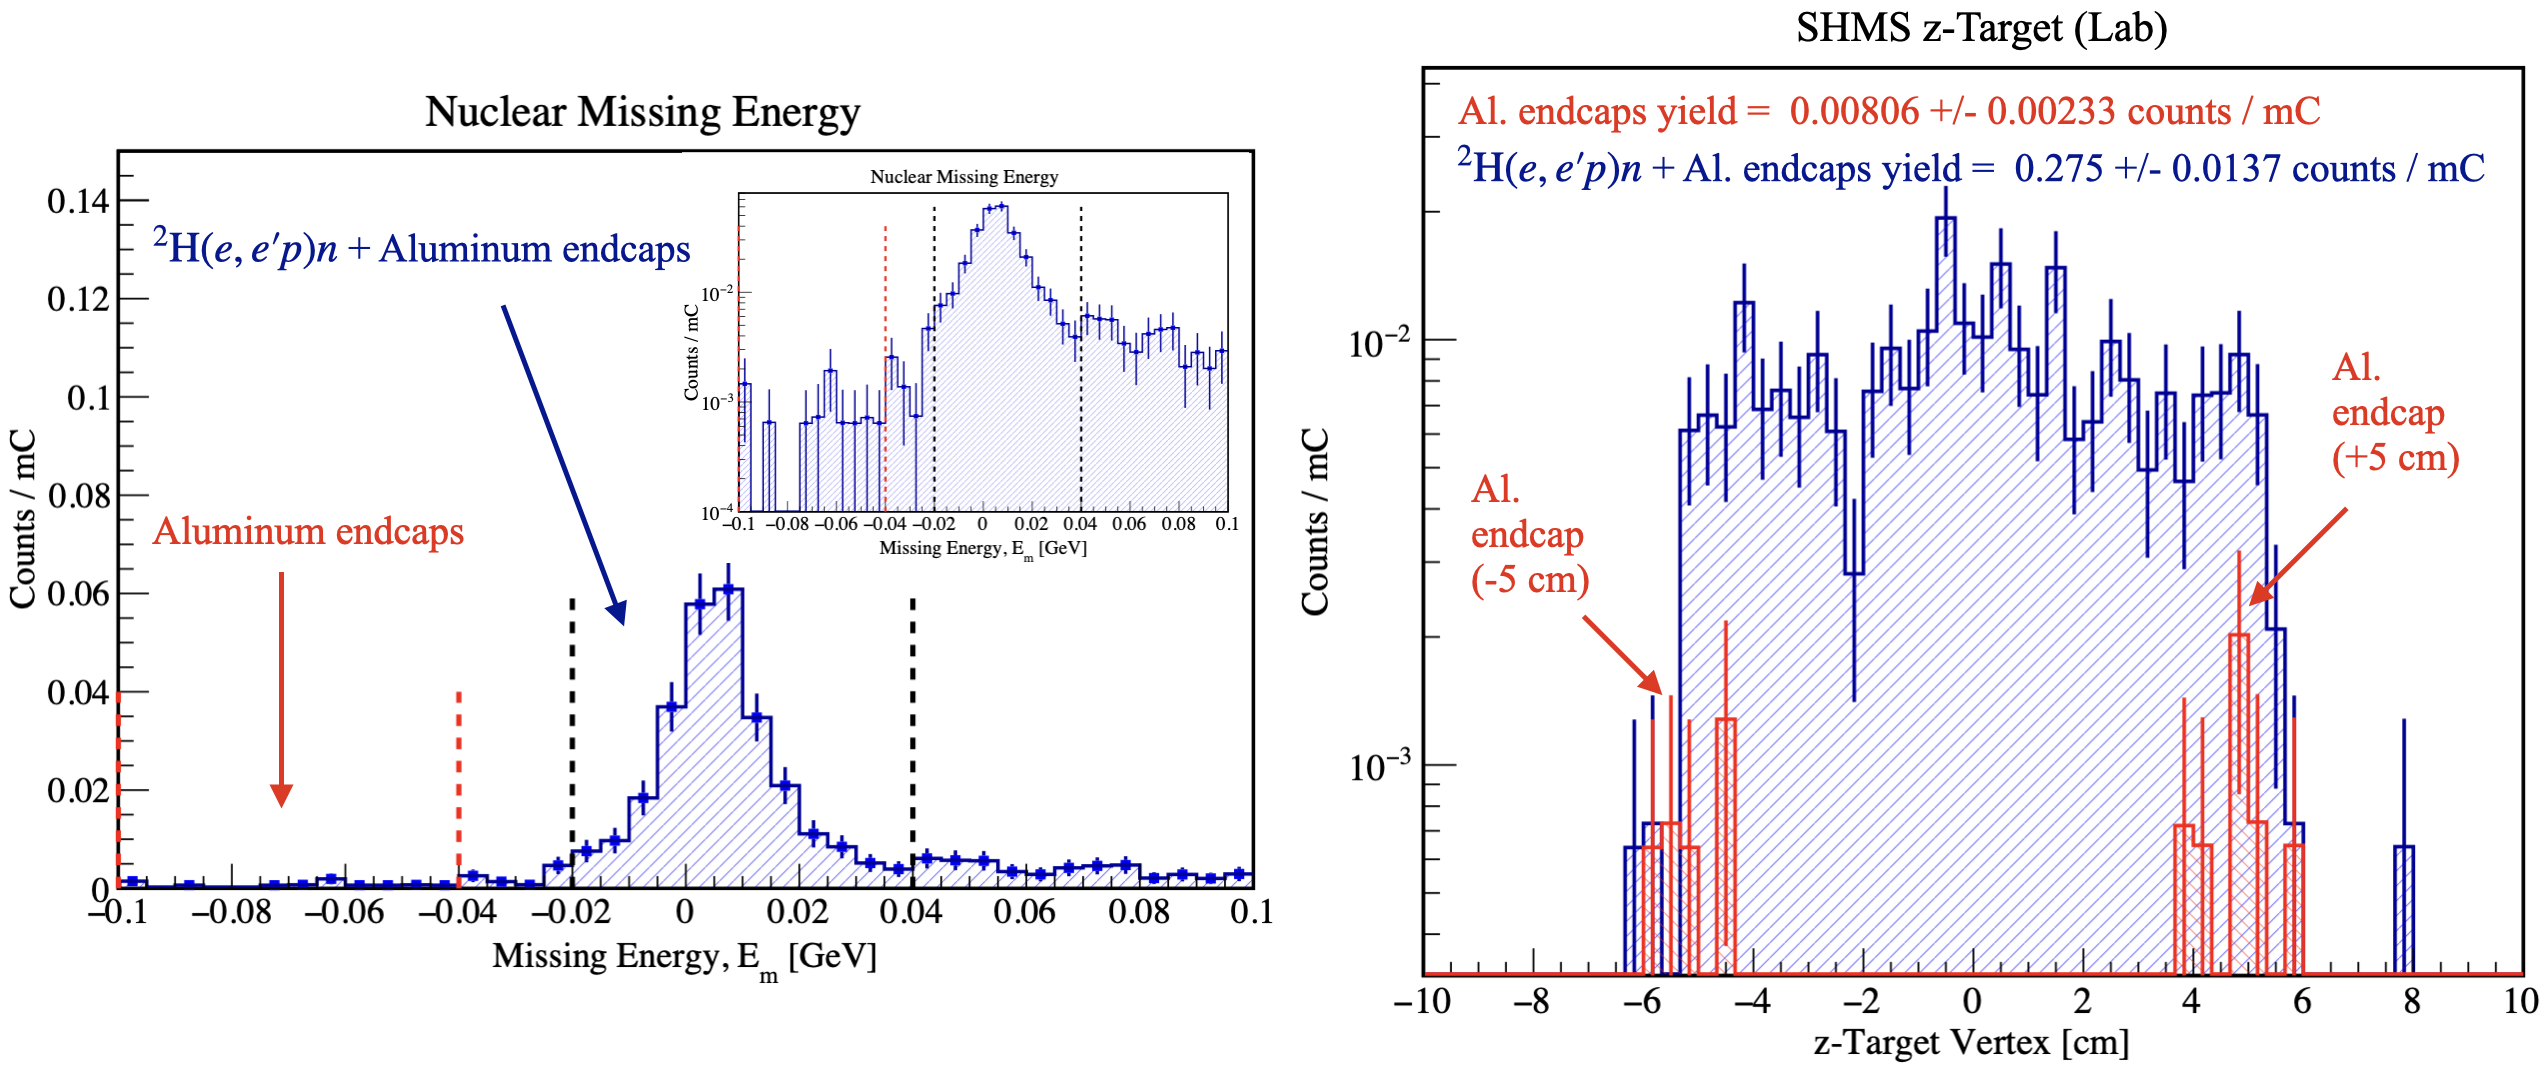
\includegraphics[scale=0.35]{plots/tgt_bkg_d2_pm580_allthnq.png}
\caption{(left) Missing energy spectrum for the deuteron 580 MeV/c setting with event selection region corresponding to Aluminum endcaps (in red) and deuteron missing energy peak over
  a 40 MeV range, each. (right) The SHMS $z$-reaction vertex corresponding to the specified region in the missing energy spectrum. Inset (left): Missing energy spectrum on a logarithmic
  scale.}
\label{fig:fig8}
\end{figure}
\section{\large Radiative \& Bin-Centering Corrections}
\noindent The radiative corrections were applied by multiplying the ratio of non-radiative to radiative SIMC yields to the data yield for each ($\theta_{nq}$,$p_{\mathrm{r}}$)
kinematic bin as described in the Letter. The radiative correction factors for $\theta_{nq}=35^{\circ}$ and $45^{\circ}$ are shown in Fig. \ref{fig:fig9}. The calculation was done using the
Laget PWIA and FSI models for systematic effect studies, but the FSI model was ultimately used to correct the data yield.
\begin{figure}[!h]
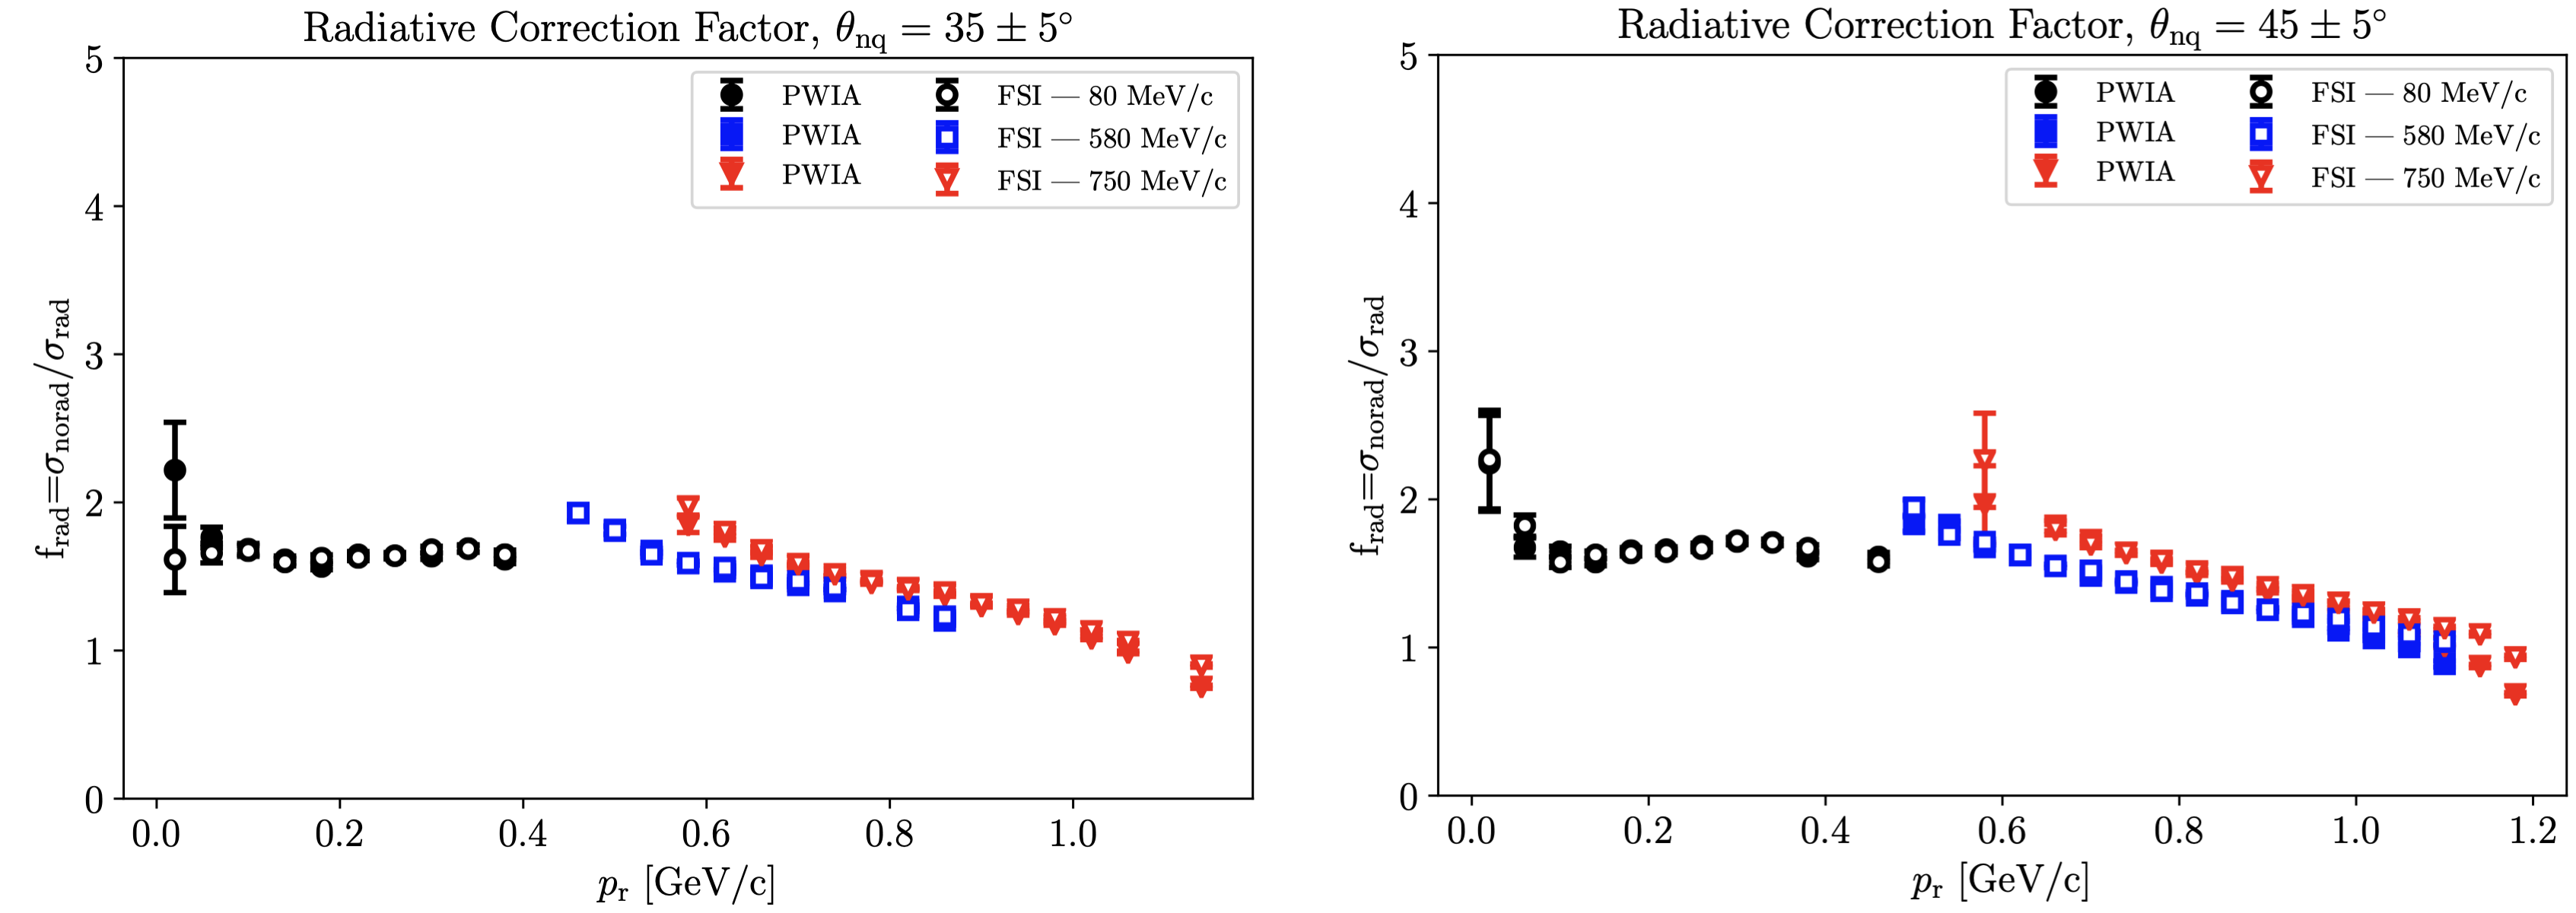
\includegraphics[scale=0.40]{plots/RC_factor.png}
\caption{Radiative correction factor versus neutron recoil momenta, $p_{\mathrm{r}}$, for $\theta_{nq}=35^{\circ}$ (left) and $45^{\circ}$ (right). }
\label{fig:fig9}
\end{figure}\\
The bin centering corrections were applied by multiplying the ratio, $f_{bc} \equiv \sigma_{avg.kin}/\bar{\sigma}$, to the average data cross section over each ($\theta_{nq}$,$p_{\mathrm{r}}$)
kinematic bin, as described in the Letter. The bin centering correction factors for $\theta_{nq}=35^{\circ}$ and $45^{\circ}$ are shown in
Fig. \ref{fig:fig10}. The calculation was done using the Laget PWIA and FSI models for systematic effect studies, but the FSI model was ultimately used to correct the data cross section.
\begin{figure}[!h]
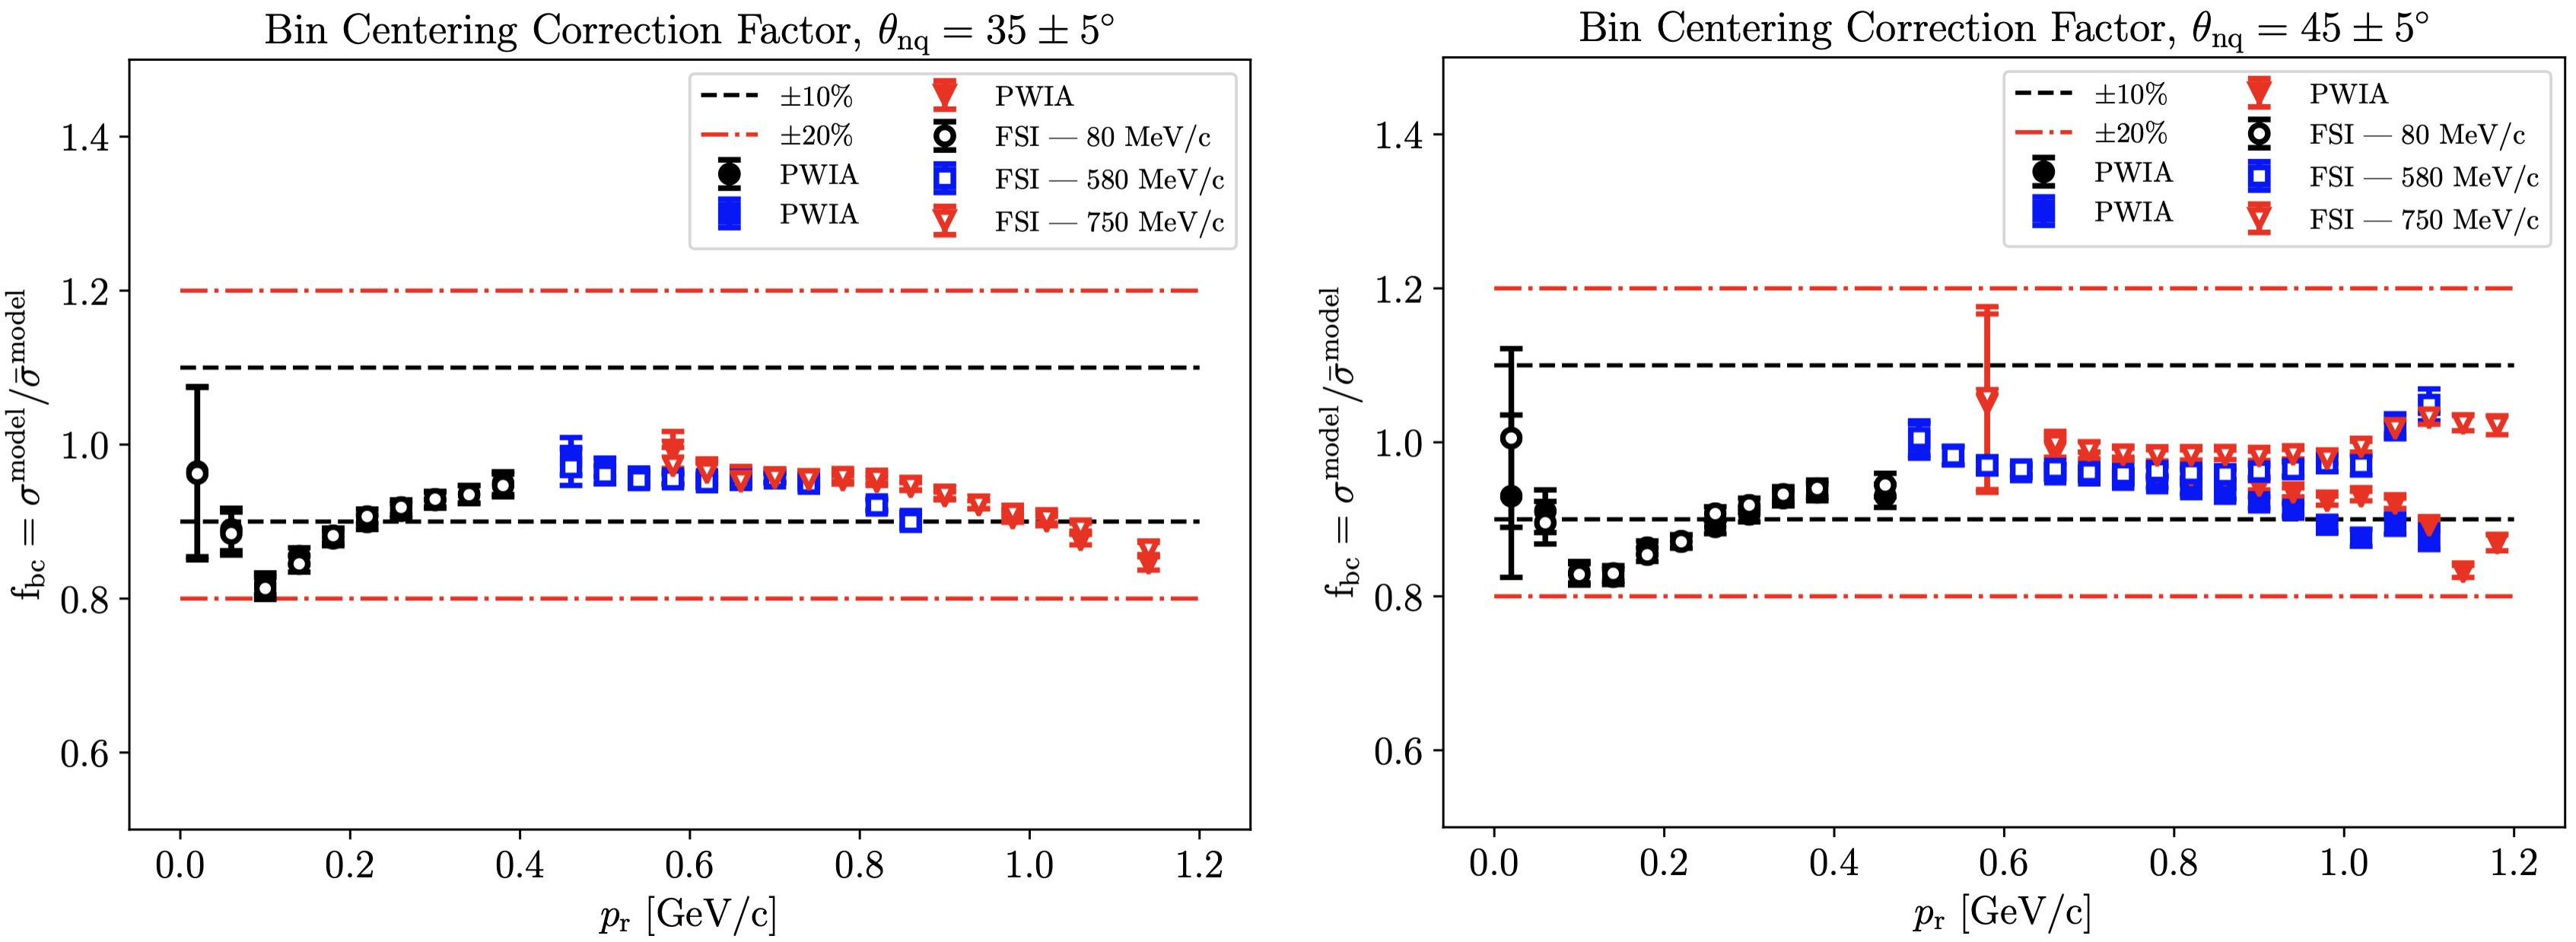
\includegraphics[scale=0.40]{plots/BC_factor.png}
\caption{Bin centering correction factor versus neutron recoil momenta, $p_{\mathrm{r}}$, for $\theta_{nq}=35^{\circ}$ (left) and $45^{\circ}$ (right).
  The inner (black dashed) and outer (red dash-dotted) lines represent a percent deviation from unity of $\pm10\%$ and $\pm20\%$, respectively.}
\label{fig:fig10}
\end{figure}
\section{\large Systematic Uncertainty Studies on Event Selection Cuts}
A study of the sensitivity on the experimental cross section due to variations in the event selection cuts was carried out. 
To determine if the variation in each of the cuts contributes to a systematic effect and whether this contribution is significant
enough to be considered as a systematic error, we used the approach by R. Barlow described in Ref. \cite{barlow2002systematic}.\\
\indent Consider a cross section measurement done two different ways (i.e., apply different cuts). Let the measurements and their
statistical uncertainties be: ($\sigma^{\mathrm{exp}}_{\mathrm{bc,1}}\pm\delta\sigma^{\mathrm{exp}}_{\mathrm{bc,1}}$) and ($\sigma^{\mathrm{exp}}_{\mathrm{bc,2}}\pm\delta\sigma^{\mathrm{exp}}_{\mathrm{bc,2}}$)
where one of the measurements is a subset of the other. The difference and its associated uncertainty can be expressed as,
\begin{subequations}
  \begin{align}
    &\Delta \equiv \sigma^{\mathrm{exp}}_{\mathrm{bc,1}} - \sigma^{\mathrm{exp}}_{\mathrm{bc,2}}, \\
    &\sigma^{2}_{\Delta} \equiv (\delta\sigma^{\mathrm{exp}}_{\mathrm{bc,1}})^{2} - (\delta\sigma^{\mathrm{exp}}_{\mathrm{bc,2}})^{2},
  \end{align}
\end{subequations}
where the error of the difference between the two measurements is found by taking the difference of their variance. As demonstrated in Ref.\cite{barlow2002systematic}, this
error accounts for the possible correlation between the two measurements. By taking the ratio
\begin{equation}
  R_{\mathrm{Barlow}} \equiv \frac{\Delta}{\sigma_{\Delta}},
\end{equation}
a criterion imposed on $R_{\mathrm{Barlow}}$ determines whether the difference is significant enough to be considered as a systematic error or sufficiently small that it may be
ignored. This criterion requires knowledge of the correlation between the subsets, but in general, as suggested in Ref.\cite{barlow2017}: if $R_{\mathrm{Barlow}} < 2$ (or $\Delta <2\sigma_{\Delta}$)
the test passes and if $R_{\mathrm{Barlow}} > 4$ (or $\Delta >4\sigma_{\Delta}$), the test fails and the discrepancy must be added as a systematic error. For $2<R_{\mathrm{Barlow}}<4$, a judgement must be made.\\
\indent Figure \ref{fig:fig11} below shows an example of the systematic effects on the missing energy cut for $\theta_{nq}=35^{\circ}$ and $45^{\circ}$ over the full $p_{\mathrm{r}}$ range.
In Fig. \ref{fig:fig11}, the different color groups represent the Barlow ratio evaluated at difference between the subset and full missing energy cut range. For mostly the entire momentum range,
the Barlow ratio was kept within 2-4 standard deviations with the exception of a few outliers which can be understood from the fact that these might have very similar variances. These systematic
studies were mainly done to check the stability of the event selection cuts and the effects of cut variation on the cross section were found to be negligible. Similar plots for the other event selection
cuts can be found in Section 5.10 of Ref. \cite{cyero_phdthesis}. 
\clearpage
\begin{figure}[!ht]
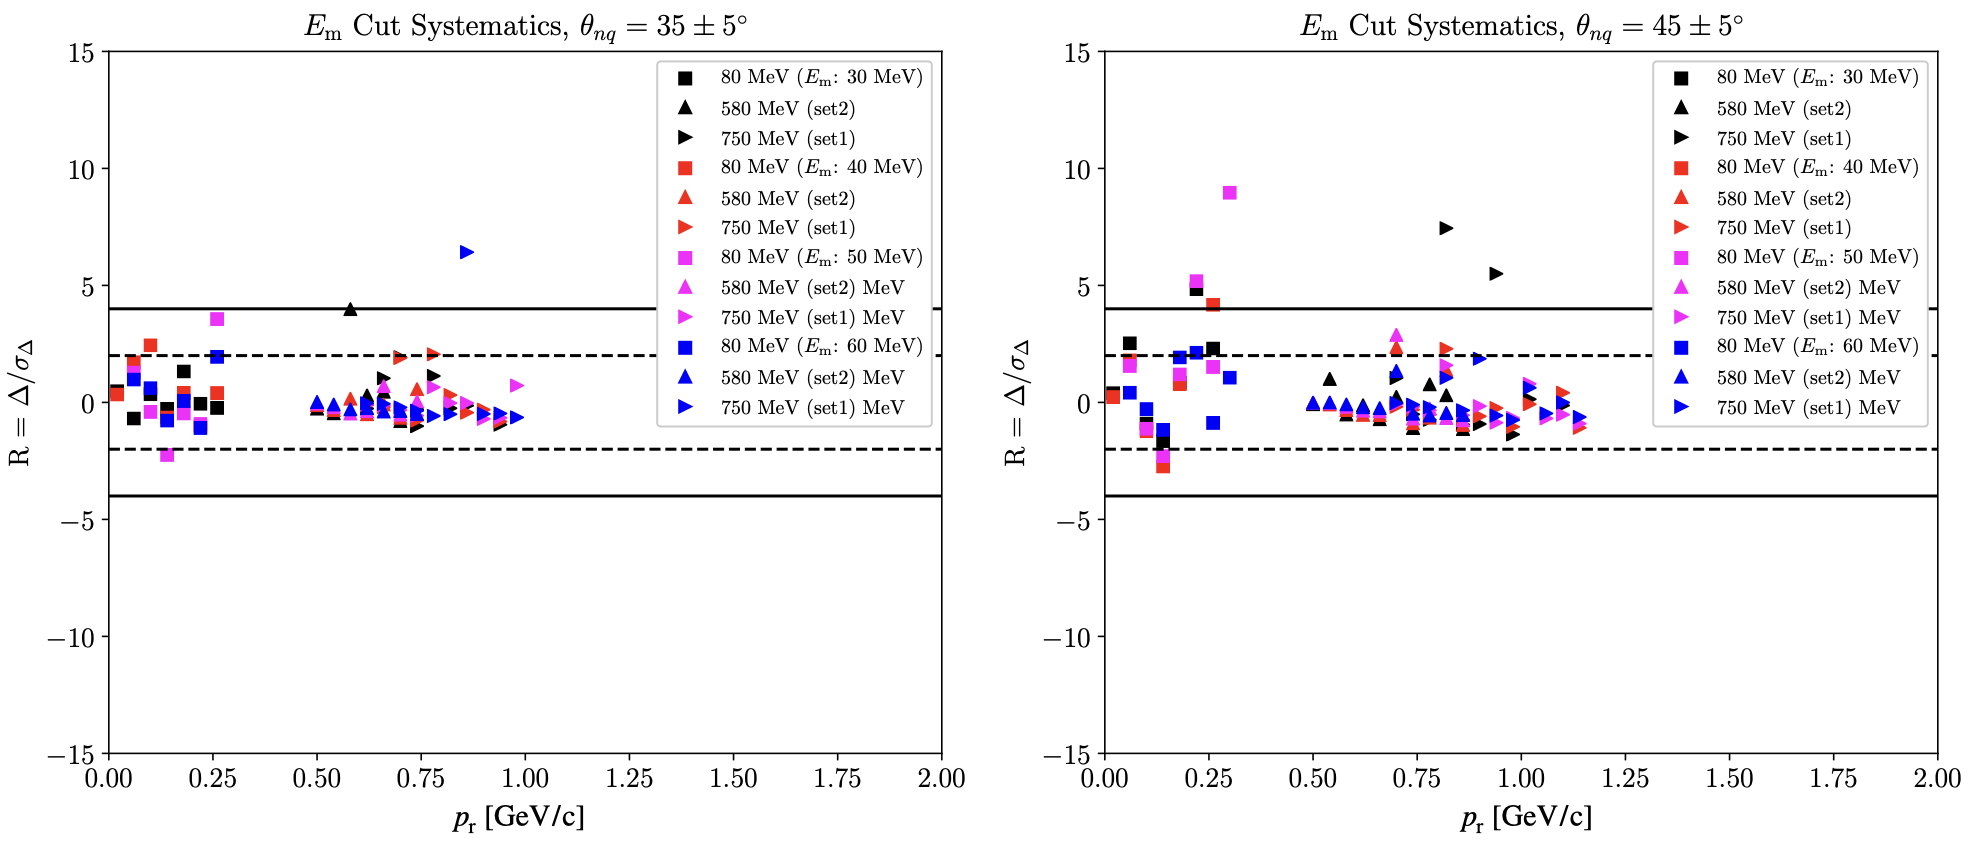
\includegraphics[scale=0.45]{plots/Em_syst.png}
\caption{Systematic effects of the missing energy cut on the data cross section for $\theta_{nq}=35^{\circ}$ (left) and $45^{\circ}$ (right). The inner (black dashed) and outer (black solid)
  lines represent the $\Delta=\pm2\sigma_{\Delta}$ and $\pm4\sigma_{\Delta}$ boundaries, respectively.}
\label{fig:fig11}
\end{figure}
\section{\large Cross-Section Extraction}
\noindent The average experimental cross section was extracted by taking the ratio of the radiative corrected data yield ($Y_{\mathrm{corr}}$) to the Monte Carlo generated phase space volume for each
kinematic bin in ($\theta_{nq}$, $p_{\mathrm{r}}$). For illustration purposes, Fig. \ref{fig:fig12} shows the experimental data yield (left) and the spectrometers' phase space volume (right) binned in
missing momentum and integrated over all $\theta_{nq}$ bins for each of the three central momentum settings.  A detailed discussion of how the experimental and reduced cross sections were extracted can be
found in Sections 5.1 and 6.1 of Ref. \cite{cyero_phdthesis}.
\begin{figure}[!h]
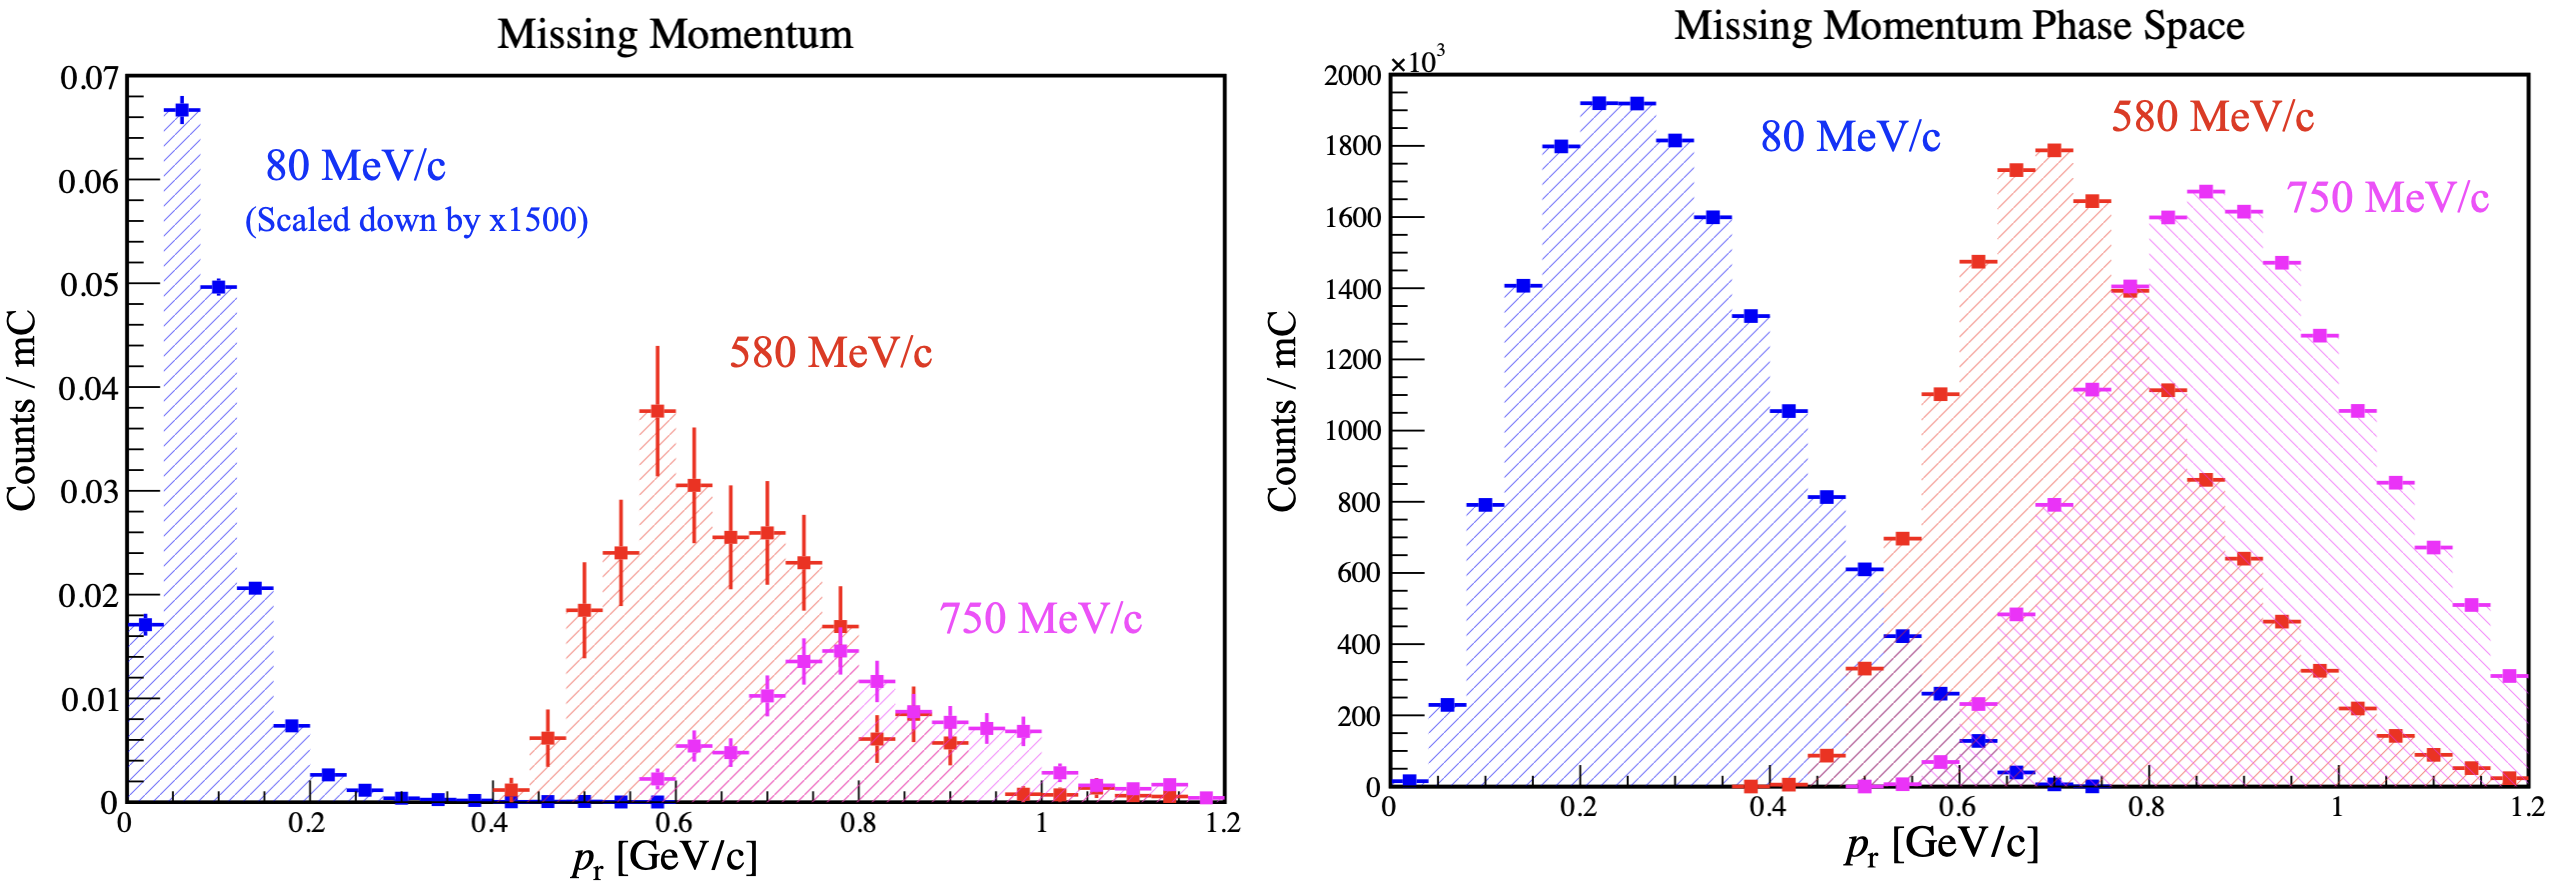
\includegraphics[scale=0.38]{plots/Pr_and_Ps.png}
\caption{(left) Experimental neutron recoil (``missing'') momentum distribution for each of the three central settings. (right) Monte Carlo (un-weighted) events generated over
  the spectrometers' phase space volume binned in missing momentum.}
\label{fig:fig12}
\end{figure}
\clearpage
\bibliography{supp}

\end{document}
